\section{\uppercase{Methodology}} \label{sec:methodology}
\subsection{Motivation} \label{sec:proposal}

Cointegration vectors can be found applying the Johansen method which uses a
sample of the last historical data. However, VECM assumes cointegration vectors do not change in time.
In fact, the long-run relationships between the time series might change due to
several economic factors that can lead to structural breaks in the cointegration
relationship \cite{gregoryETal1996}. 
In order to show the number of cointegration vectors which depends on 
the amount $L$ of historical data and the number of lags $p$ in the VECM, we used a grid search. We defined a grid of possible values for $L$ and $p$. $L$ goes throughout $[100,5000]$ with a step size of 300 and $p$  throughout $[1,5]$ with step size of 1. The first experiment consisted in determining the number of cointegration vectors for all combinations of $L$ and $p$.
We used four forex rates: EURUSD, GBPUSD, USDCHF and USDJPY with 10-second frequency. Data started at 13:00 GMT of the 13th of August 2014,
when the New York and London financial markets opened.

Figure~\ref{fig:hists} shows the distribution of the number of cointegration vectors 
given by the Johansen method for different values of $L$ and $p=1$ . This procedure was carried out by a sliding window of historical data moving 1000 times.



\begin{figure}[!h]
  %\vspace{-0.8cm}
  \centering
  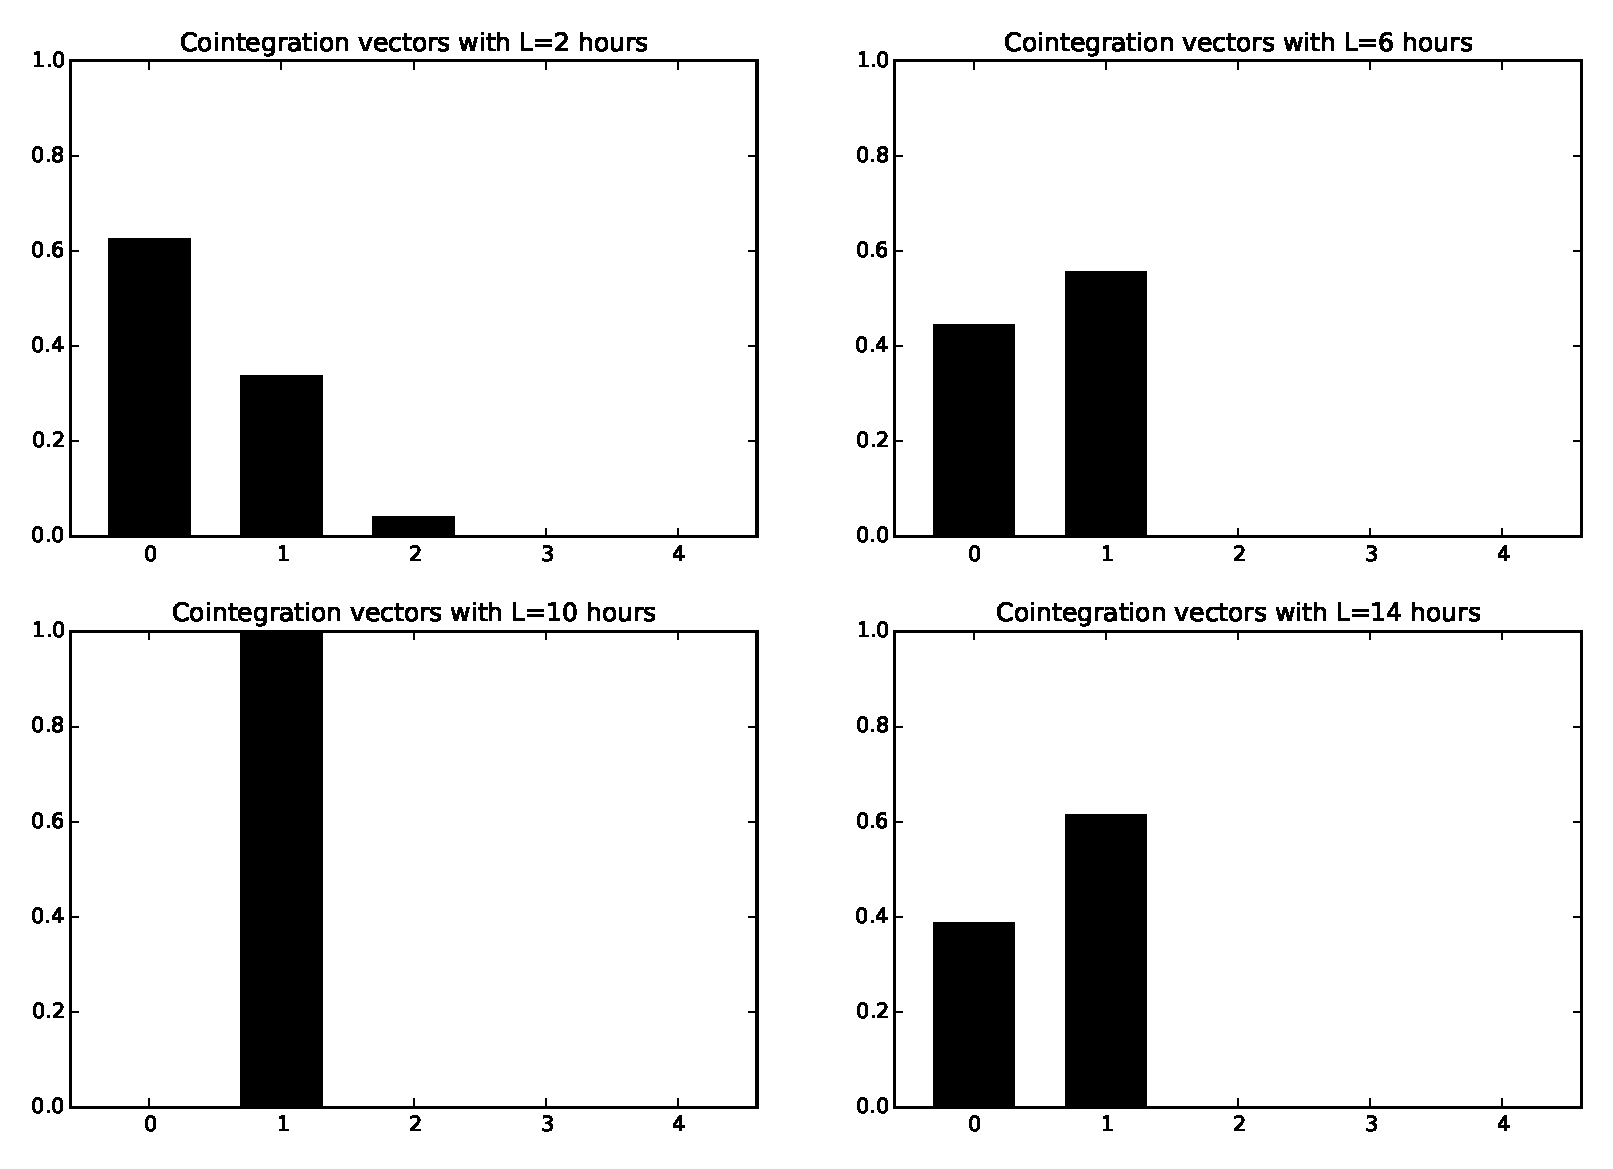
\includegraphics[width=0.9\textwidth]{img/histCointVectors-offset15000-p-1-freq-10s}
  \caption{Histogram of the number of cointegration vectors using $p=1$. Four
  possible values for $L$ are shown (100, 2000, 3000 and 4000).}
  \label{fig:hists}
\end{figure}


From section \ref{sec:background} we know that $r=0$ means no cointegration and $r=l$ (we are using four rates, so $l=4$) reveals that no process is I(1) but stationary.
The interesting cases of cointegration are those where $r$ lies strictly
between $0$ and $4$, i.e. $0<r<4$.

In order to measure the extent of cointegration, we introduce a
{\em percentage of cointegration\/} as following:
\begin{equation} \label{eq:pcoint}
PC = 
\frac{\#\{ it \mid \text{$it$ has $r$ c.v. with $0<r<l$}\}}
     {\#it}\times 100
\end{equation}
where c.v. stands for cointegration vectors and $it$ is the number of iterations.
 
The corresponding PC values for $L = [100, 2000, 3000, 4000]$ and $p=1$ (figure  \ref{fig:hists}) are: $PC = [21.3, 98.7, 79.8,  65.2]$. For the same values of $L$ and $p=3$ (figure  \ref{fig:histsp3}) the percentage of cointegration is $PC = [18.4, 92.5, 68,  52.5]$. From these results we observed that the number of cointegration vectors changed with different values for $L$ and $p$ and the percentage of cointegration depends mainly on $L$. 


The goal of our next experiment was to find a relation between this ratio
$PC$ and the performance measure MSE (see equation 
\ref{eq:MSE}). $L$ was defined between $[100,4000]$ with step size 300 and $p$ takes values between $[1,5]$ with step size 1.  

\begin{figure}[ht!]
  %\vspace{-0.8cm}
  \centering
  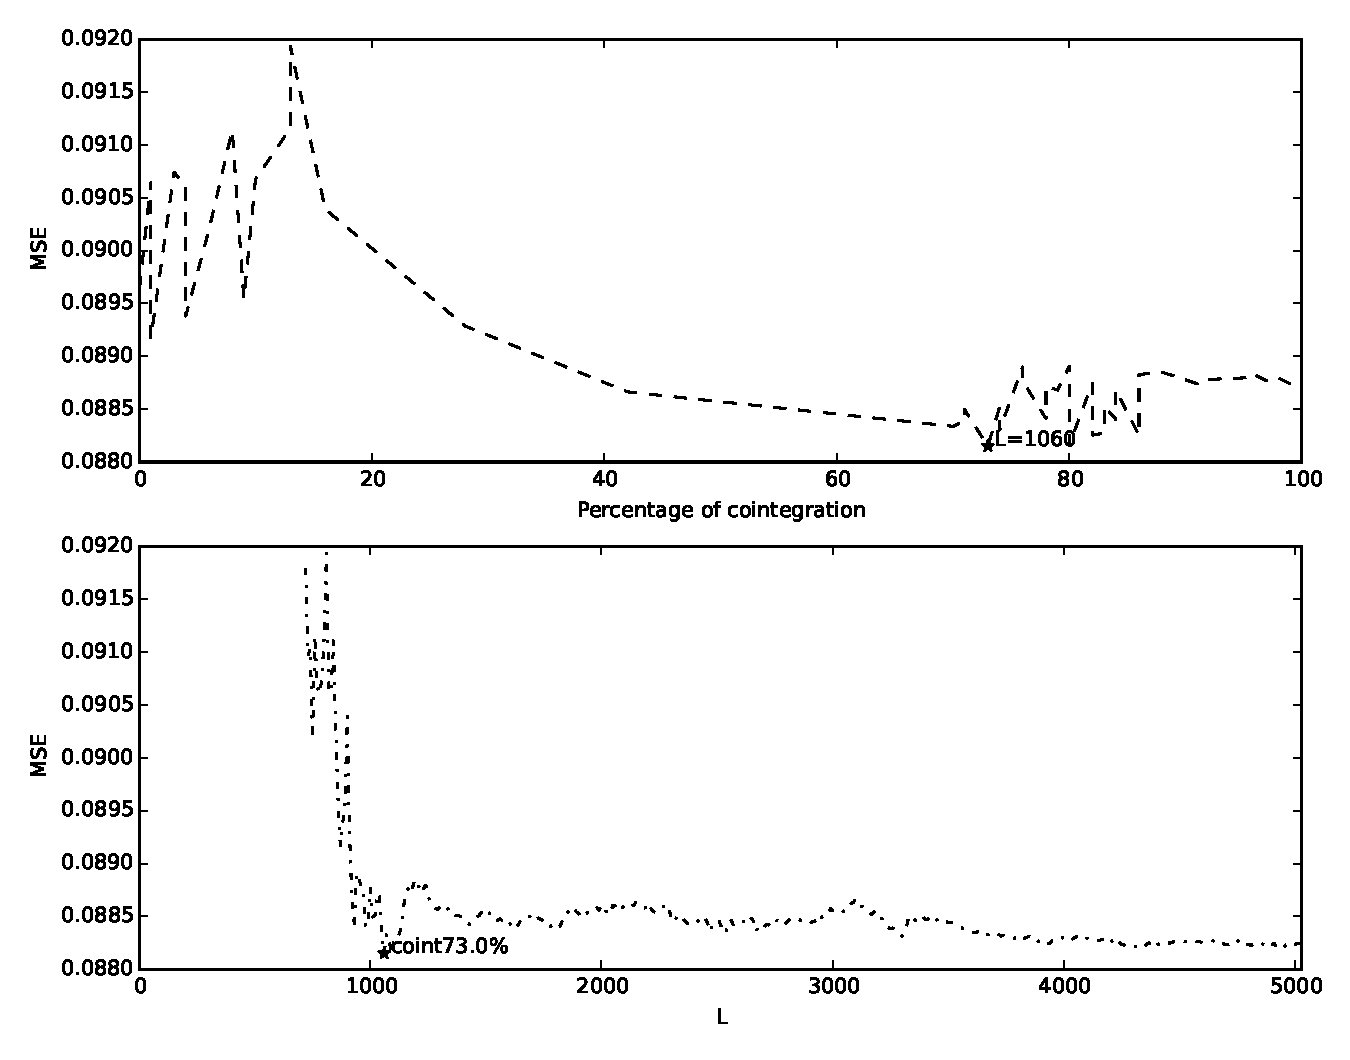
\includegraphics[width=0.8\textwidth]{img/MSE-offset20520-p-1-freq-10s}
  \caption{MSE versus the percentage of cointegration considering 1000
  iterations. Best $L$ found was 1600. Below MSE versus $L$ shows a rapidly decreasing behaviour, founding minimum at PC = 84.3\% }
  \label{fig:cointvsmse}
\end{figure}

Figure~\ref{fig:cointvsmse} shows the relation between MSE and $PC$ and $L$.
We found that better cointegration percentage leads to better
performance accuracy in terms of reducing MSE. We also found that MSE rapidly decreased with increasing $L$.

Therefore we proposed to choose $L$ and $p$ in order to maximise the percentage of
cointegration $PC$ in the near past. This process was done every time that new data was processed. However, this search can be slow if we try different values for $L$ and $p$ and therefore we distributed this calculation in order to reduce searching time.

Our proposal was then a modified version of VECM, with parameter $p$ and the amount of historical data used $L$ obtained at every step. Only the search of $L$ and $p$ was done in a distributed environment, since this is the most expensive routine. Our proposal is called Adaptive Vector Error Correction model (AVECM).
AVECM is detailed in the algorithm ~\ref{alg:AVECM} which summarises our proposal. 

\begin{algorithm}[ht!]
\begin{algorithmic}[1]
\REQUIRE $\,$ \\
$\mathbf{y}$: matrix with $N$ input vectors and $l$ time series\\
$j$: Starting point of testing \\
$it$: Ending point of testing \\
$ps$: list of $p$ values \\
$Ls$: list of $L$ values ($L<N$) \\
$m$: Iterations to determine parameters ($m < N-L$)\\
\ENSURE  $\,$ \\
$\{ \hat{\mathbf{y}}[1],\dots,\hat{\mathbf{y}}[it]\}$: prediction vectors \\
\FOR { $i =j$ to $it$ }
   \STATE $\mathbf{Y} \gets \mathbf{y}[:,i-1]$
    \STATE $L,p \gets
    \texttt{get\_best\_params}(Ls,ps,m,\mathbf{Y})$
        \STATE $model = \text{VECM}(\mathbf{Y},L, p)$
        \STATE $\hat{\mathbf{y}}[i-j] = model.predict()$
\ENDFOR
\end{algorithmic}
\caption{AVECM: Adaptive VECM.}
\label{alg:AVECM}
\end{algorithm}

The input of AVECM is time series prices which are cointegrated. The starting point of testing is $j$ and the total number of iterations is $it$. We need to ensure that $j$ is at least the maximum value of $Ls$. $Ls$ and $ps$ are the possible values for $L$ and $p$.
The function {\bf get\_best\_params} makes this grid search on the two vector
lists $Ls$ and $ps$ and returns the parameters $L$ and $p$ which maximise
the percentage of cointegration $PC$ (see equation~\ref{eq:pcoint}) for a
pre-defined number of iterations $m$. This function is implemented in a distributed 
environment, thus ensuring a response
before new data is available. 
After $L$ and $p$ parameters are found, VECM is built and used
to forecast the next data point.


\subsection{Model comparison} \label{sec:random}
We compared our proposal, in terms of performance, with the naive forecast of the random walk model and ARIMA. It is still difficult to outperform the random walk model for standard econometric forecasting models \cite{lo2011} despite its simplicity. The random walk model is defined as:

\begin{equation}
\mathbf{y}_t = \mathbf{y}_{t-1} + \epsilon_{t}
\label{rwmodel}
\end{equation}

The naive forecast of the time series difference $\hat{\mathbf{y}}_{t+1}$ for the random walk model is defined as:
\begin{equation}
\hat{\mathbf{y}}_{t+1} = \mathbf{y}_t + \hat{\epsilon}_{t+1} 
\end{equation}
\noindent where  $\hat{\epsilon}_{t+1} = \epsilon_{t}$.

On the other hand, ARIMA is widely used to forecast returns in finance \cite{tsay2005}. A process can be modelled as an ARIMA$(p,d,q)$ model if $\mathbf{x}_t=\Delta^d \mathbf{y}_t $, i.e after differencing $d$ times the time series $\mathbf{y}_t$,  we get an ARMA$(p,q)$. Since we are modelling returns, we used $d=1$.


\subsection{Evaluation methods} \label{sec:evaluation}

Forecast performance was evaluated using two different methods which are frequently used in finance:
\begin{description}
\item
{\bf MSE},  Mean Square Error measures the distance between forecasts
and the true values and large deviations from the true value have a
large impact due to squaring forecast error.
\begin{equation}\label{eq:MSE}
\text{MSE} = 
\frac{\displaystyle \sum_{t=1}^{N} (\mathbf{y}_t-\hat{\mathbf{y}}_t)^2}{N}
\end{equation}
\item {\bf $U$-statistic}, the Theil's $U$-statistic \cite{theil1966} is a unit free measure obtained as the ratio between the root MSE (RMSE) of a model and the RMSE of the naive random walk model. A $U$-statistic less than 1 implies the performance is better than the naive model.
\end{description}


